\chapter{Detecção de eventos}

A detecção de eventos consiste no processo de identificação de um evento dentro de um sistema. Um sistema, por sua vez, é uma combinação de elementos que interagem organizados para atingir um ou mais objetivos declarados \cite{ISOIEC24765}. Ou seja, um sistema é uma coleção de componentes que somente combinados atingem um objetivo final. Esses componentes podem incluir softwares e hardwares, assim como documentos, técnicas, serviços, políticas, entre outros.

Um evento é um padrão de mudança significativo ou ocorrência anômala em relação ao comportamento geral do sistema observado. Detecção de eventos, logo, envolve o que permite que ocorrências significativas sejam detectadas dentro de um sistema. Como existem vários tipos de sistemas, a detecção deve ser compatível com cada um deles para poder interagir com seus componentes, ou seja, uma técnica de deteção de eventos referente a um sistema pode não se adequar a outro, tornando cada detector único, ou compatível com apenas o nicho em que foi implementado.

As entradas de dados para a detecção de eventos também são variadas, podendo ser documentos textos, sons, imagens, vídeos, etc. Em um texto, por exemplo, a detecção pode ter o fim de detectar o repentino surgimento de palavras-chave em uma gama de documentos. Em imagens, a detecção pode ser utilizada para detectar se houve um rompimento de alguma barreira por algum objeto intruso. Ou ainda, em publicações coletadas de um serviço de rede social, para utilizar as atividades dos usuários para detectar eventos que ocorrem no mundo real.

O sistema de detecção de eventos deve ser capaz de transformar os dados vindo dos sensores e identificar os eventos inerente à esses dados. Os dados dos sensores são dados de baixo-nível, sendo medições diretas de uma característica do mundo, e a detecção deve transformá-lo em dados de alto nível, ou seja, análises nas quais seja possível a compreensão humana. Para realizar esse fato, o algoritmo deve agregar, converter e reformatar os dados recebidos em uma estrutura que é independente da fonte de dados \cite{Fienberg2005}.

Como a detecção de eventos é precisamente acoplada ao sistema em questão, existem muitos métodos para a sua implementação. Eles podem ser categorizados entre métodos estatísticos, métodos probabilísticos e métodos de aprendizado de máquina. 

\begin{itemize}
	\item \textbf{Métodos estatísticos:} analisam a coleção de dados obtidos a fim de aplicar modelos que possam prever os estados e deduzir estados passados do sistema a fim de detectar eventos relevantes. 
	\item \textbf{Métodos probabilísticos:} utilizam os dados para criar modelos probabilísticos para prever em qual categoria uma nova entrada será classificada. 
	\item \textbf{Métodos de aprendizado de máquina:} utilizam técnicas para criar relações entre os dados obtidos e deduzir a classificação de uma nova entrada.
\end{itemize}

Para o modelo implementado, é utilizada a detecção de eventos em documentos de texto previamente coletados do serviço de rede social Twitter utilizando o método de aprendizado de máquina \textit{máquina de vetores de suporte}. 

\subsection{Eventos e Sistemas}

Eventos são resumidamente definidos por \citeonline{Allen1994}:

\begin{quote}
[..] eventos são primariamente cognitivos ou linguísticos por natureza. Ou seja, o mundo não contém eventos. Ao invés, eventos são os meios que agentes classificam informações e padrões de mudança relevantes.
\end{quote}

Portanto, um evento é um conceito cognitivo, que depende de cada sistema implementado. Por exemplo, um evento para o sistema de monitoramente da velocidade de um carro, é o carro chegar à determinada velocidade. Um sistema de monitoramento de ocorrências de doenças a partir de relatórios médicos, é uma subida no número de casos de uma determinada doença. E assim é para cada caso específico, ou seja, cada construção de sistema irá determinar o que é um evento para ele específico. 

Um evento pode ser, então, a erupção repentina de determinado termo em uma gama documentos, uma medida fora do padrão de temperatura, pressão, altura de voz, objeto em uma imagem, frequência de palavras-chave, etc. Por esse fator de subjetividade e de acoplação com o sistema em questão, para cada sistema os eventos serão representados de maneiras diferentes. Segundo \citeonline{Jiang2009}, sistemas podem ser categorizados das seguintes maneiras:

\begin{itemize}
	\item \textbf{Natural x artificial:} Em sua classificação mais básica, sistemas podem ser de origem natural ou artificial. Sistemas naturais são os sistemas já presentes na natureza, já os artificiais são os criados pelo homem.
	\item \textbf{Observável x não-observável:} Sistemas observáveis são os que suas características podem ser observadas pelo homem, sem a necessidade de um sensor específico, como monitorar se está dia/noite. Não-observáveis necessitam da implementação de um sensor específico, como monitorar se a temperatura de um ambiente está acima de 40ºC.
	\item \textbf{Qualitativo x quantitativo (método de análise):} Sistemas podem ser analisados de qualitativamente ou quantitativamente. Na primeira, o sistema é analisado de acordo com suas saídas diretamente. No segundo, de acordo com a medição de performance ou métricas derivadas das saídas do sistema.
\end{itemize}

No modelo implementado, os eventos são detectados em um sistema artificial, não-observável e analisados qualitativamente. Sistemas não-observáveis, por sua vez, necessitam de \textit{sensores}, para quantificar os dados do ambiente e permitirem a detecção de eventos.

\section{Sensores}

Para a detecção de eventos dentro de sistemas não-observáveis, são utilizados sensores, que são os componentes que quantificam e medem as informações presentes no ambiente em questão. Por exemplo, em um sistema de monitoramento de temperatura, o sensor mede a temperatura do ambiente e a quantifica, gerando dados de baixo-nível que podem ser manipulados e analisados. As saídas dos sensores são utilizadas como entrada no sistema de detecção de eventos. 

Sensores também podem ser das mais variadas naturezas, como de temperatura, velocidade, pressão, altura, etc. Porém, os sensores são quaisquer componentes produtores dos dados e quantificadores do ambiente analisado. Um canal de publicações de notícias pode ser um sensor, na medida que o sistema de detecção de eventos analise seus documentos de texto como formato de entrada de dados, com o possível de detectar repentinos surgimentos de novos tópicos. Ou relatórios médicos, para detecção de erupção de doenças, etc.

Um sensor pode, ainda, ser um usuário de um serviço de rede social, ao criar uma publicação sobre um determinado acontecimento, possibilitando a aplicação da detecção de eventos para detectar este determinado acontecimento dentro de uma gama de outras publicações. O sensor, nesse âmbito, é denominado como \textit{sensor social}.

Os recursos são os insumos para a implementação da detecção de eventos, podendo ser os dados gerados diretamente pelos sensores - a atual medida de temperatura, velocidade, uma publicação etc - ou através de algum dado indireto considerado relevante. Um sistema que possui um sensor de pressão como gerador de recursos, um recurso indireto relevante pode ser quanto tempo o sensor passou com a pressão acima de um determinado valor.

\subsection{Detecção de eventos em documentos de texto}

As entrada de dados para detecção de eventos podem ser dos mais variados formatos, um deles são documentos de texto. A técnica é implementada para analisar padrões presentes nos documentos, com o fim de detectar se os mesmos contem referências à eventos do mundo real, ou seja, se está presente naquele documento a menção à algum evento ocorrido. Um evento, nesse caso, indica uma ocorrência significativa e também um evento do mundo real, tal como shows, festas, eventos esportivos, políticos etc.

Segundo \citeonline{Weng2011}, os métodos existentes para a implementação da técnica de detecção de eventos em documentos de texto podem ser classificadas em dois tipos: documento-pivô e recurso-pivô. 

Os métodos de \textit{documento-pivô} baseiam-se na divisão de documentos em grupos de acordo com a similaridade léxica entre os mesmos, porém, como não existe regra para implementação da detecção, também não existe padrão para a criação dos algoritmos. \citeonline{Yang1998} apontam alguns padrões que ajudam a produzir os algoritmos:

\begin{itemize}
	\item \textbf{Proximidade temporal:} Documentos referentes ao mesmo evento costumam ser próximos temporalmente, sugerindo o uso combinado de similaridade léxica e proximidade temporal como critério para a clusterização.
	\item \textbf{Erupção de documentos similares:} O espaço de tempo entre a erupção de documentos similares geralmente indica eventos diferentes, sugerindo o monitoramento da clusterização ao longo do tempo.
	\item \textbf{Mudança de frequência:} Rápidas mudanças na frequência de um termo geralmente apontam para documentos referentes à um novo evento, indicando a importância de atualizar a coleção de palavras e seus pesos na clusterização.
\end{itemize}

Os métodos de \textit{recurso-pivô}	analisam a distribuição e a associação entre palavras-chave. Não existe também um jeito considerado melhor para se implementar, e cada caso precisa ser analisado em sua unicidade, porém \citeonline{Sakaki2010} citam três grupos de recursos para a implementação do método:

\begin{itemize}
	\item \textbf{Recursos estatísticos:} O número de palavras em um documento e a posição da palavra-chave dentro do mesmo.
	\item \textbf{Recursos de palavras-chave:} As palavras presentes no documento
	\item \textbf{Recursos de contexto de palavra:} As palavras antes e depois da palavra-chave.
\end{itemize}

Segundo \citeonline{Aiello2013} ambos os métodos possuem vantagens e desvantagens. Os métodos de documento-pivô possuem problemas com a fragmentação de grupos e, em um contexto de aquisição de documentos em tempo real, eles dependem de limiares arbitrários para a inclusão de um documento em um grupo. Já os métodos de recurso-pivô geralmente fazem associações errôneas entre palavras-chave.

\section{Serviços de redes sociais e sensores sociais}

Os serviços de redes sociais (SNS: \textit{Social Networking Services}) são plataformas online em que os usuários podem se relacionar criando perfís, compartilhando publicações e atualizações nos formatos de texto, foto, vídeo, etc. Com a migração das pessoas para os ambientes virtuais, os SNSs possuem grande atração de usuários. O Facebook, atualmente o serviço com maior base de usuários, possui mais de 1 bilhão de contas cadastradas.

Os SNS se tornaram a principal forma com que as pessoas se relacionam online e compartilham informações sobre a sua vida e suas experiências. Diariamente, são criadas milhões de publicações nos principais serviços disponíveis, sobre os mais variados temas e acontecimentos, tornando esses serviços grandes fontes de pesquisa e monitoramento de informação.

Os maiores serviços disponíveis possuem interfaces para desenvolvedores, em que fornecem as informações geradas por seus usuários abertamente, para que esses dados sejam adquiridos e analisados de forma sistemica. Isso possibilita a análise  criação de vários tipos de serviços externos que se conectam aos servidores dos SNS e obtem os dados gerados por seus usuários e os analisam para os mais variados fins. Um dos serviços externos pode ser utilizado para a detecção de eventos que, segundo \citeonline{Dong2014}, é um dos tópicos mais importantes na \textit{análise de redes sociais}.

A \textit{análise de redes sociais} é uma análise metódica de redes sociais através da aplicação de técnicas de mineração de dados. Segundo \citeonline{Olowe2014}, além da detecção de eventos, outras técnicas constituem em:

\begin{itemize}
	\item \textbf{Detecção de comunidades:} Uma comunidade é uma um pequeno grupo dentro de uma grande rede. A formação de comunidades é uma das características mais importantes dos serviços de redes sociais e técnicas de \textit{clusterização} são utilizadas para detectá-las.
	\item \textbf{Análise e formação de opinião:} A análise de opinião consiste no descobrimento e reconhecimento de expressões positivas ou negativas sobre um determinado assunto de interesse. As opiniões podem influenciar a decisão de outros usuários e a formação de opinião pode ser analisada através de técnicas de clusterização, para analisar o impacto que opiniões tem nas redes analisando nós afetados e não afetados.
	\item \textbf{Definição e sumarização de opinião:} A definição de opinião pode ser encontrada em um texto, frase ou documento. A sumarização utiliza a técnica de \textit{máquina de vetores de suporte} para somar todas as diferentes opiniões de um documento analisando a polaridade, o grau e as ocorrências das opiniões.
	\item \textbf{Análise de sentimentos:} Análise de sentimentos pode ser expressada como o descobrimendo e reconhecimento de opiniões positivas ou negativas sobre determinadas empresas, produtos, serviços, eventos, etc. É utilizada para criar ferramentas de suporte de decisão e ajudar entidades a tomar decisões necessárias.
\end{itemize}

Relacionados aos SNS estão os \textit{microblogs}, uma maneira de compartilhar informação no formato de texto curto, que permite que os usuários façam rápidas atualizações, sendo o mais popular entre eles o Twitter. No entanto, o microblog é um conceito, então outras ferramentas também o implementam, como Facebook, Google+, entre outros na forma de \textit{atualização de status}, que é uma forma do usuário compartilhar rapidamente o que está pensando. O Twitter possui o diferencial de ser focado no recurso de microblog, podendo usufruir de todas as suas principais características.

Pelo tamanho reduzido das publicações, nos microblogs o esforço necessário para a geração de informação é menor, o que potencializa e adiciona dinamismo ao compartilhamento de experiências entre usuários, facilitando que a informação publicada se espalhe rapidamente. Ao vivenciar um evento, o usuário pode sentir, imediatamente, a necessidade de compartilhar com seu grupo de amigos, e publicar em seus microblogs se mostrou como o jeito escolhido para esse fim. Por sua característica pessoal e de tempo real, eles se tornam uma fonte única de informação sobre todo os tipo de acontecimentos do mundo \cite{Mai2012}. 

O usuário, ao realizar uma publicação em seu microblog, passa a atuar verdadeiramente como um sensor de acontecimentos do mundo real. Assim como sensores físicos como o de temperatura, localização ou proximidade, o usuário, ao vivenciar um acontecimento e publicar sobre ele, está agindo como um \textit{sensor social} do mesmo. Ou seja, se ele cria uma mensagem no serviço sobre a ocorrência de uma manifestação ao seu redor, então pode-se considerar que, como um ``sensor de manifestações'', ele está exibindo um valor positivo. A Figura 2.1 representa o usuário como sensor de acontecimentos do mundo real e produtor de documentos que são armazenados serviço do Twitter, criando publicações sobre eventos naturais, eventos esportivos, desastres não-naturais, etc.

\begin{figure}[htpb]
	\begin{center}
		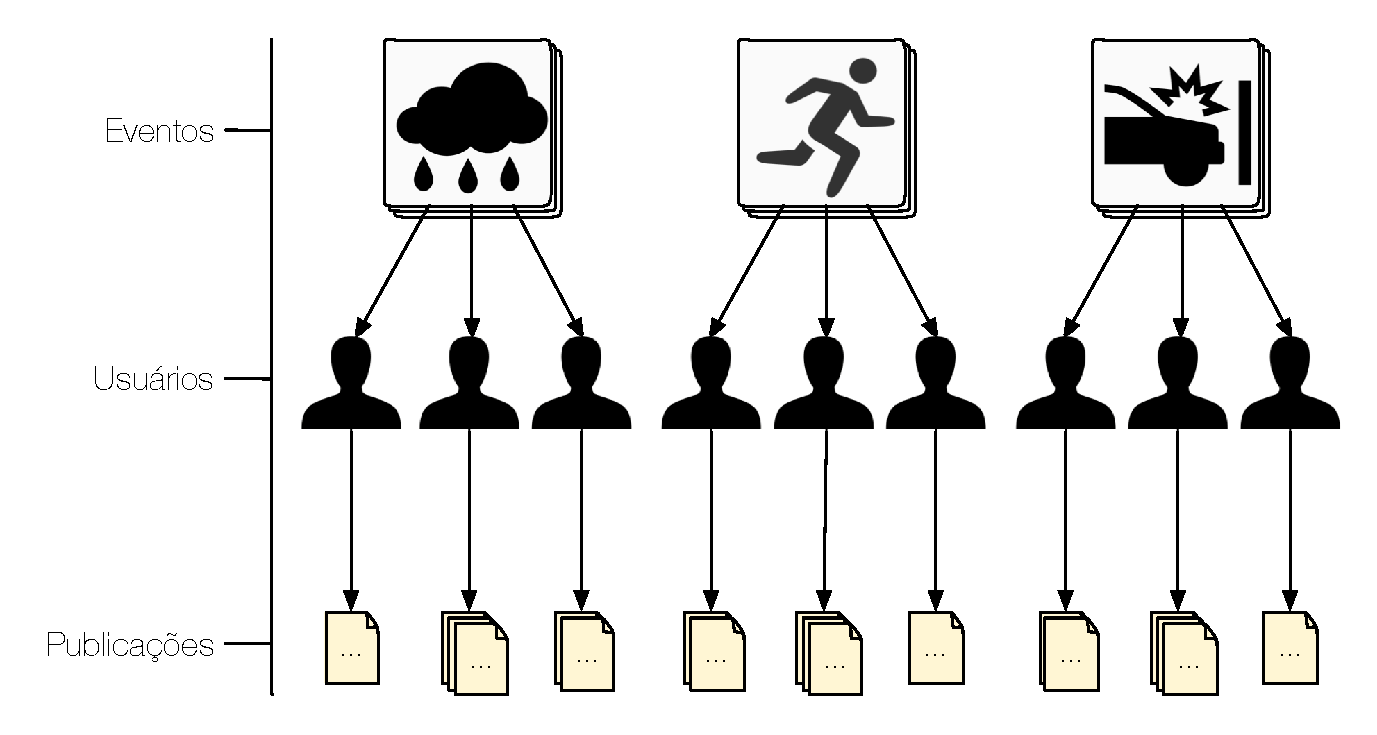
\includegraphics[width=0.85\textwidth]{figuras/event-perception-2.eps}
		\caption{O usuário como sensor de eventos do mundo real.}
	\end{center}
\end{figure}

Apesar da característica principal dos SNS ser a possibilidade dos usuários se relacionarem, cada serviço possui suas características específicas. Os principais serviços da atualidade são Twitter, Facebook Google+, etc.

\subsubsection*{Twitter}

O Twitter é um serviço de microblog aonde os usuários interagem entre si compartilhando publicações de texto limitadas até 140 caracteres. A principal característica do serviço é o dinanismo das publicações e a sua facilidade de compartilhamento. O dinanismo do serviço é explicitado pela funcionalidade de \textit{trending topics} (assuntos do momento), aonde estão ranqueados os termos mais comentados do momento, sendo atualizado várias vezes por dia.

A principal forma de interagir com outros usuários no Twitter através do recurso \textit{seguir}. Ao seguir um usuário, você passa a receber todas as suas publicações na sua página de \textit{linha do tempo}. A linha do tempo é principal página de interação com o sistema, aonde são exibidas todas as publicações dos usuários que você segue. Para cada publicação é possível \textit{curtir} (gostar publicamente), responder ou \textit{retweetar} (publicar novamente a mensagem para os usuários te seguem). Na Figura 2.2 está apresentada a linha do tempo de um usuário. No primeiro bloco da coluna da esquerda estão as informações do usuário ``Augusto'', sua quantidade de publicações, quantoas pessoas ele segue e quantas estão o seguindo. No segundo bloco estão os \textit{assuntos do momento}. Na coluna da direita se encontra a \textit{linha do tempo}.

\begin{figure}[htpb]
	\begin{center}	
		\includegraphics[width=0.8\textwidth]{figuras/twitter-main-screen.eps}
		\caption{Página principal do Twitter: linha do tempo.}
	\end{center}
\end{figure}

Hoje, com mais de 500 milhões de usuários registrados, o serviço criado em 2006 por Jack Dorsey cresce exponencialmente e tem ganhado atenção em várias frentes de pesquisas acadêmicas, exatamente por sua característica de troca de informações em tempo real. O trabalho de \citeonline{Java2007} apresenta a formação de comunidades e qual a motivação das pessoas ao utilizarem os serviços de microblogs e o Twitter, e concluiu que essa forma de interação induz à alta reciprocidade e correlação, indicando um entendimento mútuo entre os usuários e a facilidade de pulverização de informação. \citeonline{Jansen2009} estudaram o uso do Twitter como uma ferramenta de transferência de informação de pessoa para pessoa e analisou que o Twitter é uma das peças chave para o monitoramento de informação. \citeonline{Matuszka2013} analisam o ciclo de vida de cada palavra-chave com fim de detectar eventos, e enfatizam que o aparecimento de eventos específicos em redes sociais podem surgir antecipadamente aos outros meios de comunicação. \citeonline{Gao2014}, em seu trabalho, estuda o Twitter e os assuntos do momento, e uma forma de sumarizá-los e de retenção de informações e histórias, para que elas não se percam devido à intensa criação de informações proporcionada pelo serviço. 

O Twitter possui interfaces abertas para que aplicações externas sejam criadas. É possível através de serviços externos publicar por um usuário, ver todas as suas publicações, gostar de uma publicação, entre diversas outras ações. Através das interfaces, também é possível a busca por palavras-chave, o que torna o Twitter um serviço interessante para aplicação de diversas técnicas. Com ela é possível que serviços externos façam buscas complexas e recebam, em tempo real ou não, as publicações criadas por usuários correspondentes à essa busca. Tornando possível que se obtenha uma enorme quantidade de publicações para que sejam feitas análises de forma automatizada de dados, como a detecção de eventos.

\subsubsection*{Facebook}

O Facebook é o serviço de rede social mais popular da atualidade, e conta com cerca de 1.3 bilhão de usuário únicos\footnote{http://www.statisticbrain.com/facebook-statistics/}. O serviço possui várias maneiras de ser utilizado, ultrapassando o âmbito da conexão entre amigos e familiares. Além de ser possível criar seu perfil, compartilhar e visualizar publicações de texto, fotos e vídeos e criar amizades (conexões) com amigos, familiares e colegas de trabalho, o serviço oferece também a possibilidade da criação de páginas específicas para estabelecimentos comerciais, figuras famosas, organizações não governamentais etc. Também é possível a criação de eventos e convidar amigos, grupos privados e secretos e uma gama de outras coisas.

O serviço foi criado por Mark Zuckerberg em 2004 e vem crescendo rapidamente todos os anos. Hoje, cerca de 3 milhões de publicações são enviadas a cada 20 minutos e 2 milhões de novas conexões entre amigos são solicitadas\footnote{http://www.statisticbrain.com/facebook-statistics/}. O Facebook é, sem dúvida, a rede social com mais atividade entre seus usuários.

O Facebook possui a poderosa interface para desenvolvedores chamada Graph API, que é a principal ferramenta com que se interage de forma sistêmica com o serviço. É uma interface baseada em HTTP que pode ser utilizada para consultar dados, realizar publicações, subir fotos, etc. A Graph API é baseada em três princípios\footnote{https://developers.facebook.com/docs/graph-api/quickstart/v2.0}:

\begin{itemize}
	\item \textbf{Nós:} Entidades como Usuário, Foto ou Comentário.
	\item \textbf{Bordas:} As conexões entre as entidades, como fotos de um usuário, ou comentários de uma foto.
	\item \textbf{Campos:} Informações sobre as entidades, como o nome de um Usuário ou data de criação de uma foto.
\end{itemize}

A Graph API, porém, não permite com que sejam consultadas as publicações no serviço no âmbito geral, ou seja, com ela é possível apenas buscar as publicações ou realizar atividades relacionadas à um usuário em específico. Para realizar buscas por publicações através de palavras-chave, por exemplo, é necessário utilizar a \textit{Keyword Insights API} ou a \textit{Public Feed API}, porém, essas APIs são liberadas apenas para um conjunto específico de editores de mídia e não é possível, atualmente, conseguir chave para utilização das mesmas.

\subsubsection*{Google+}

O Google+ (Google Plus) é o serviço de rede social criado pelo Google Inc. em 2011. Hoje, após a incorporação dos usuários de outros serviços do Google como Gmail e Orkut, o serviço conta com uma base de cerca de 1.1 bilhão de usuários\footnote{http://socialmediaslant.com/google-plus-traffic-stats-february-2014/}.

O Google+ possui muitas das suas funcionalidades inspiradas no serviço Facebook, seu principal concorrente, porém com o diferencial de ser baseado em círculos de amizade. Nos círculos você pode compartilhar publicações apenas para um determinado grupo de amigos ou familiares, além de permitir a melhor organização de todas as pessoas que conhece. 	

O serviço possui interface para desenvolvedores chamada \textit{Google+ API}, que é possível com que se integre aplicativos e sites com o mesmo, podendo realizar publicações, criar amizades, obter informações de usuários, etc. Porém, possui a limitação de que apenas é possível buscar informações relacionadas à um usuário em específico e suas ligações. O serviço não disponibiliza uma interface com que seja possível buscar publicações de modo geral, como o Twitter oferece.

\section{Métodos de detecção de eventos}

Os métodos para implementação da técnica da detecção de eventos podem ser categorizados em métodos estatísticos, métodos probabilísticos e métodos de aprendizado de máquina. Segundo \citeonline{Jiang2009}, embora existam outros métodos que não se encaixam nessas categorias, a maioria pertence à uma ou mais delas.

\subsection{Métodos estatísticos}

O método estatístico mais simples consiste na aplicação de um \textit{limiar} superior ou inferior em que, caso o dado vindo do sensor chegue a esse limiar o evento é detectado, como no caso do velocímetro do carro. Porém, os valores observados geralmente dependem dos valores passados, necessitando de métodos que representem esses estados passados e possam fazer previsões futuras, como os métodos de \textit{regressão}, \textit{séries temporais} e \textit{filtro de kalman}.

No método de análise e modelagem de \textit{regressão}, a variável dependente (Y) é modelada como uma função de variáveis independentes (X) e um termo de erro, que representa a variação da variável dependente que não pode ser explicada pelo modelo. O modelo de regressão linear é expressado pela Figura 2.3, em que os pontos são os valores exatos da variável dependente (Y) e a reta significa a aproximação estatística por regressão linear. Porém, quando quando a relação entre a variável dependente e a independente é observadamente não-linear, é necessário criar modelos de regressão não-lineares.

\begin{figure}[htpb]
	\begin{center}
		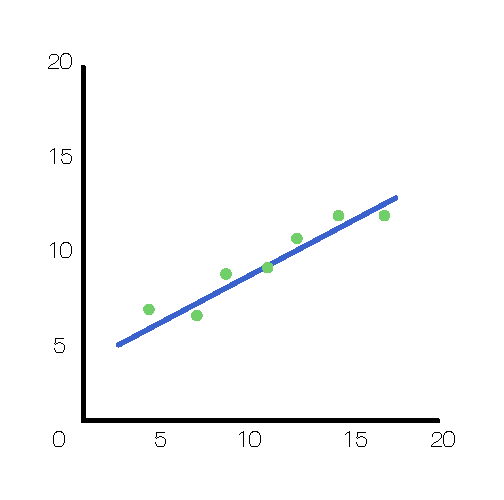
\includegraphics[width=0.4\textwidth]{figuras/regressao-linear.eps}
		\caption{Modelo de regressão linear.}
	\end{center}
\end{figure}

O método de \textit{séries temporais} consiste na modelagem estatística de dados que são medidos sucessivas vezes, com o mesmo intervalo de tempo entre as medições. O método tem como objetivo modelar os processos estocásticos subjacentes aos dados encontrados, para poder prever o valor de um estado futuro ou passado.

O \textit{filtro de Kalman} é um método estatístico recursivo criado por Rudolf Kalman que utiliza das medições ao longo do tempo para gerar predições que se aproximem de estados futuros e passados.

\subsection{Métodos probabilísticos}

Métodos probabilísticos, ao invés de analisarem e testarem amostras de dados como nos métodos estatísticos, consistem na estimativa da probabilidade da ocorrência de um evento e outras probabilidades e parâmetros relacionados. Existem diversos modelos e distribuições probabilísticas, como as de \textit{Poisson} e de \textit{Bernoulli}.

O modelo de \textit{Poisson} é utilizado quando se deseja calcular a probabilidade a ocorrência de um evento em um determinado espaço de tempo, sendo que os mesmos ocorrem independentemente e que a probabilidade de um evento ocorrer não muda através do tempo.

O modelo de \textit{Bernoulli} é utilizado quando os recursos analisados são binários, como por exemplo, a presença ou ausência mesmo. O modelo calcula a probabilidade de uma saída pertencer à uma classe ou outra.	

\subsection{Métodos de aprendizado de máquina}
	
Os métodos de aprendizado de máquina são geralmente utilizados quando os sensores são distruibuídos de forma esparsa no espaço e no tempo. Esses métodos geralmente recebem grandes volumes de informação e requerem alto poder computacional. Alguns exemplos são os \textit{filtros de partículas} e \textit{máquina de vetores de suporte}.

Os \textit{filtros de partículas} são algoritmos de aproximação probabilística que implementam o filtro Bayes. Em eventos, a técnica é utilizada para a estimativa de localização através de distruibuições probabilísticas que se propagam no tempo. Para isso, são geradas hipóteses (partículas) da localização de acordo com a distribuição dos dados. Por exemplo, para determinar a posição de um avião no espaço, sabendo sua posição em relação ao solo e a topologia do solo, o algoritmo, baseando-se nessas informações, gera inúmeras hipóteses de onde o avião possa estar. No próximo instante de tempo, sabendo a velocidade do avião e a sua direção, as possibilidades são atualizadas, até que as hipóteses convergirem para um valor considerado aceitável.

As \textit{máquinas de vetor de suporte} (SVM: \textit{support vector machines}) são algoritmos de aprendizado de máquina utilizados para a classificação de dados, que os analisam e reconhecem padrões. Eles são capazes de classificar futuras entradas a partir da análise de um conjunto de dados amostra previamente classificados.

No SVM, cada nova entrada de dados é representada como um ponto em um espaço, em que a técnica consiste em achar a divisão desses pontos que possui a maior margem possível entre eles, indicando assim a separação das duas classes. Na Figura 2.4 está ilustrada a maneira com que um SVM linear classifica as entradas de dados em dois grupos, porém esta classificação não é geralmente feita em um espaço de duas dimensões, e sim em um espaço de altíssima dimensão, podendo ser também feita de forma não-linear.

\begin{figure}[htpb]
	\begin{center}
		\includegraphics[width=1.0\textwidth]{figuras/svm-two-dimensional-field.eps}
		\caption{Classificação de um SVM: maior margem possível entre os dois grupos.}
	\end{center}
\end{figure}

Os SVMs são muito utilizadas para a detecção de eventos em documentos de texto, por funcionarem bem com um grande número de recursos, poucos recursos irrelevantes, dados esparsos e por conta da maioria dos problemas de classificação de texto serem lineares \cite{Joachims1998}.

\section{Classificação de texto}

A detecções de eventos em documentos de texto se apoia na técnica de \textit{classificação de texto}, que consiste na categorização de documentos em grupos aplicando um conjunto de técnicas que podem ser variadas, de acordo com o problema em questão. Segundo \citeonline{Aggarwal2012}, a classificação de texto pode ser aplicada nas mais variadas áreas, como:

\begin{itemize}
	\item \textbf{Organização e filtro de notícias:} Portais de notícias nos quais existe a criação de um grande volume de artigos todos os dias utilizam a classificação de texto - chamado nessa área também de filtragem de texto - para categorizar e filtrar os artigos de forma automatizada, pois em muitos casos a organização manual é inviável.
	\item \textbf{Organização e obtenção de documentos:} Muitos métodos de classificação de texto podem ser aplicados também em outras áreas, como bibliotecas digitais, literatura científica e publicações de redes sociais, com o fim de organizar os documentos de texto e facilitar sua futura obtenção.
	\item \textbf{Mineração de opinião:} A técnica pode ser aplicada para revisar avaliações de consumidores, geralmente pequenos textos, para determinar informações importantes para as empresas interessadas.
	\item \textbf{Classificação de email e filtro de spam:} A técnica pode, também, ser aplicada para classificar emails, para determinar se o email em questão é relevante ou apenas spam.
\end{itemize}

Os algoritmos para a classificação de texto precisam ser capazes de lidar com grandes quantidades de dados. Os textos podem ser modelados de acordo com suas palavras e as frequências das mesmas, logo, os algoritmos devem suportar dados que são esparsos, de alta dimensão e com baixa frequência na maioria das palavras. 

A maioria dos métodos de detecção de eventos podem ser encontrados e aplicados na classificação de texto. Segundo \citeonline{Aggarwal2012}, além das \textit{máquinas de vetores de suporte}, outros métodos mais utilizados são:

\begin{itemize}
	\item \textbf{Árvores de decisão:} As árvores de decisão são implementados criando uma divisão hierárquica dos textos, de acordo com os recursos especificados previamente. De acordo com cada recurso, é escolhido se o texto se enquadra no mesmo ou não, sendo possível, então, determinar à qual classe o texto pertence.
	\item \textbf{Classificadores baseados em padrões:}	Os classificadores baseados em padrões são implementados separando os textos em classes de acordo com seus padrões de palavras. Cada padrão de palavras aponta para uma classe, e esses padrões são utilizados para a classificação.
	\item \textbf{Classificadores Bayesianos:} Os classificadores bayesianos são classificadores probabilísticos baseados nos recursos de palavras de cada classe. Os textos analisados são classificados de acordo com a probabilidade deles pertencerem à uma classe específica.
\end{itemize}

A representação dos documentos e a seleção de recursos são questões importantes para a implementação dos métodos para classificação de texto. 

Os documentos podem ser representados como um conjunto de palavras, não importando a sua ordem, ou um conjunto de frases, em que cada documento é uma sequência de palavras. A maioria dos métodos de classificação de texto utilizam os documentos como um conjunto de palavras, por sua simplicidade de implementação.

A seleção dos \textit{recursos} pode ser feita através da remoção de palavras-filtradas (\textit{stop-word removal}) ou da redução de palavras-filtradas (\textit{stop-word stemming}). No primeiro, as palavras que não indicam as diferentes classes são removidas. No segundo, as palavras que possuem alguma relação pré-definida são reduzidas à apenas uma palavra, como remoção de plurais e de prefixos ou sufixos.

\section{Trabalhos Relacionados}

Os trabalhos de detecção de eventos encontram aplicação nos mais variados âmbitos. Muitos trabalhos aplicaram métodos estatísticos para comparar os resultados entre seus modelos e as atuais medições dos sensores como forma de detectar eventos anômalos. Outros aplicaram métodos probabilísticos para categorizar as medições em grupos de interesse. Outros utilizaram métodos de aprendizado de máquina para treinar e categorizar futuras ocorrências. E muitos outros aplicaram uma ou mais dessas técnicas no âmbito do Twitter.

\citeonline{Gupchup2009} utiliza a técnica de Análise de Componente Principal (PCA) para construir um modelo que é capaz de coletar as tendências das medidas de uma rede de sensores sem fio, e então são analisadas as diferenças entre o modelo e as reais medidas dos sensores para detectar anomalias. \citeonline{Hong2014} utilizam a detecção de eventos para detectar intrusos em redes de computadores. \citeonline{Zleikha2014} desenvolvem um algoritmo de decisão de floresta aleatória (random forest) para detectar eventos em dados vocais. Os eventos em questão podendo ser momentos de silêncio, risadas, etc.

\citeonline{Soule2005} desenvolveram um detector de eventos para detectar anomalias em redes de larga escala como empresas ou provedores utilizando filtro de kalman para filtrar o tráfego de rede comum e, para o tráfego remanescente são aplicadas quatro técnicas. Uma foca no comportamento instantâneo, outra na mudança da média do tráfego remanescente, a terceira em mudanças o comportamento da variância e a quarta nas mudanças da variância em múltiplas escalas de tempo.

No trabalho de \citeonline{Ihler2006} é construído um modelo de Poisson variável no tempo para detectar eventos anômalos em dados de contagem de séries temporais. A utilidade do modelo é demonstrada em dois âmbitos, dados de rodovias e de acessos à construções, e observa que o modelo possui melhor performance que um modelo não-probabilístico baseado em limiar. Os resultados indicaram que o modelo fornece uma robusta e precisa ferramenta para aprendizado autônomo e adaptável para separar eventos não usuais de atividades normais.

O trabalho de \citeonline{Sakaki2010} desenvolveu um algoritmo que detecta terremotos e tufões no Japão através das publicações coletadas do Twitter. As palavras ``terremoto'' e ``tremendo'' são utilizadas como palavras-chave, e foi utilizado o método de aprendizado de máquina \textit{máquina de vetores de suporte} com o kernel linear. O conjunto de amostras inicial que alimentou o SVM para a análise semântica foi composto por 597 publicações e depois da aquisição de resultados positivos, a localização e o horário de um terremoto são estimados utilizando os métodos probabilisticos filtro de kalman e filtro de partículas. Como resultado foi produzida uma notável aplicação, que detecta 96\% dos terremotos com escalas de intensidade 3 ou maior no território do Japão.

Um sistema que monitora publicações e detecta ocorrências de rinite alérgica no Japão foi desenvolvido por \citeonline{Takahashi2011}. A aplicação monitora publicações que contém a expressão ``hay fever'' (rinite alérgica) enviadas ao Twitter e utiliza o algoritmo AdaBoost.SDF, criado por \citeonline{Iwakura2008}, para classificar as publicações. Foi necessária a utilização do dado da localização do perfil do usuário para estimar a localização das publicações, e a normalização do número de publicações para cada região do Japão também foi necessária, pois percebeu-se que o número de publicações criadas em regiões em que o Twitter era popular era muito superior à outras áreas. Ao analisar a correlação entre os dados obtidos pelos sensores sociais e pelos sensores já utilizados, \citeonline{Takahashi2011} chegaram a conclusão de que o Twitter pode ser utilizado, neste caso, como uma alternativa aos sensores já existentes.

Um trabalho de investigação foi feito por \citeonline{Mai2012}, que analisou se as publicações enviadas ao Twitter pode ser uma fonte de dados para acidentes de transporte. O trabalho utiliza a API de transmissão em tempo real do Twitter para detectar publicações relevantes contendo palavras-chave como ``acidente'', ``batida'', ``rodovia'' e apenas as publicações contendo a localização geográfica do usuário foram selecionadas. Essas publicações são então comparadas com o os dados do orgão da Califórnia \textit{California High Patrol} utilizando os métodos de comparação baseado em volume e semântico. Concluiu-se que existe correlação entre os dados extraídos das publicações analisadas e os dados do órgão da California, porém um sofisticado filtro de conteúdo e localização se mostrou necessário para maximizar a relevância dos dados.

\citeonline{Wang2013} desenvolveram um algoritmo para a detecção de palavras que erupcionam repentinamente no Twitter. As palavras são obtidas através da interface para desenvolvedores \textit{Streaming API}. É utilizado o pré-processamento de palavras para remover replicações como risadas ou onomatopéia. A remoção de palavras de filtragem é utilizada e publicações com menos de duas palavras também são filtradas. É utilizado um probabilístico de mistura Gaussiano para a extração das palavras que erupcionam e para a detecção de evento. Finalmente, para o reconhecimento da localização é utilizado um modelo probabilístico de campo aleatório condicional (CRF: \textit{conditional random field}).

\section{Discussão das técnicas}

\citeonline{Wang2013} utiliza a interface para desenvolvedores do Twitter \textit{Streaming API}, porém, optamos por utilizar a interface \textit{REST API} pois com ela é possível obter publicações mais antigas e não necessitar da manutenção de uma conexão que fique sempre ativa. A \textit{Streaming API}, como é um serviço de tempo real, aceita apenas novas obtenções de publicações a partir do momento seguinte à conexão.

Os trabalhos de \citeonline{Sakaki2010}, \citeonline{Mai2012} e \citeonline{Takahashi2011} aplicam a detecção em eventos de alto impacto como desastres naturais, acidentes de transito e doenças. Escolhemos aplicar a técnica para a detecção de eventos de manifestações por possuir características semelhantes como geração de impacto, revolta e ser um evento anômalo ao funcionamento comum da sociedade de modo geral.

Obtou-se pela utilização do SVM como classificador de texto por demonstrar alta recorrência em trabalhos como \citeonline{Santos2010}, \citeonline{Pak2010}, \citeonline{Benevenuto2010}, \citeonline{Go2009}, entre outros.